%%%%%%%%%%%%%%%%%%%%%%%%%%%%%%%%%%%%%%%%%%%%%%%%%%%%%%%%%%%%%%%%%%%%%%%%%%%%%%%%
%2345678901234567890123456789012345678901234567890123456789012345678901234567890
%        1         2         3         4         5         6         7         8

\documentclass[letterpaper, 10 pt, conference]{ieeeconf}  % Comment this line out if you need a4paper

%\documentclass[a4paper, 10pt, conference]{ieeeconf}      % Use this line for a4 paper

\IEEEoverridecommandlockouts                              % This command is only needed if 
% you want to use the \thanks command

\overrideIEEEmargins                                      % Needed to meet printer requirements.

%In case you encounter the following error:
%Error 1010 The PDF file may be corrupt (unable to open PDF file) OR
%Error 1000 An error occurred while parsing a contents stream. Unable to analyze the PDF file.
%This is a known problem with pdfLaTeX conversion filter. The file cannot be opened with acrobat reader
%Please use one of the alternatives below to circumvent this error by uncommenting one or the other
%\pdfobjcompresslevel=0
%\pdfminorversion=4

% See the \addtolength command later in the file to balance the column lengths
% on the last page of the document

% The following packages can be found on http:\\www.ctan.org
\usepackage{graphics} % for pdf, bitmapped graphics files
\usepackage{epsfig} % for postscript graphics files
%\usepackage{mathptmx} % assumes new font selection scheme installed
%\usepackage{times} % assumes new font selection scheme installed
\usepackage{amsmath}
\usepackage{amssymb}  % assumes amsmath package installed
%\usepackage[hidelinks]{hyperref}
\usepackage{hyperref}
\usepackage{subcaption}
%\usepackage{array}
\usepackage[table]{xcolor}
\usepackage{collcell}
\usepackage{hhline}
\usepackage{pgf}
\usepackage{pgfplots}
\usepackage{multirow}
\usepackage[ruled,vlined]{algorithm2e}
\usepackage{booktabs,dcolumn}
\usepackage{etoolbox,siunitx}
\usepackage{dblfloatfix}
\captionsetup{labelsep=newline,
	singlelinecheck=false,
	skip=0.333\baselineskip}
\newcommand\Tstrut{\rule{0pt}{2.0ex}}       % "top" strut

\title{\LARGE \bf
	Coverage Path Planning in Large-scale Multi-floor Urban Environments with Applications to Autonomous Road Sweeping
}


\author{Daniel Engelsons$^{1}$ and Mattias Tiger$^{1}$ and Fredrik Heintz$^{1}$% <-this % stops a space
	\thanks{}% <-this % stops a space
	\thanks{$^{1}$Daniel Engelsons, Mattias Tiger and Fredrik Heintz are with the Department of Computer and Information Science, Link{\"o}ping University, Sweden.
		{\tt\small mattias.tiger@liu.se, fredrik.heintz@liu.se}
	}%
}


\begin{document}
	
	
	
	\maketitle
	\thispagestyle{empty}
	\pagestyle{empty}
	
	
	%%%%%%%%%%%%%%%%%%%%%%%%%%%%%%%%%%%%%%%%%%%%%%%%%%%%%%%%%%%%%%%%%%%%%%%%%%%%%%%%
	\begin{abstract}
		Coverage Path Planning is the work horse of contemporary service task automation, powering autonomous floor cleaning robots and lawn mower in households and office sites. While steady progress has been made on indoor cleaning and outdoor mowing, these environments are small and with simple geometry compared to general urban environments such as city parking garages, highway bridges or city crossings. To pave the way for autonomous road sweeping robots supposed to operate in such difficult and complex environments, a benchmark suite with three large-scale 3D environments representative of this task is presented. On this benchmark we evaluate a new Coverage Path Planning method in comparison with previous well performing algorithms, and demonstrate state-of-the-art performance of the proposed method. Part of the success, for all evaluated algorithms, is the usage of automated domain adaptation by in-the-loop parameter optimization using Bayesian Optimization. Apart from improving the performance, tedious and bias-prone manual tuning is made obsolete, which makes the evaluation more robust and the results even stronger.
	\end{abstract}
	
	
	%%%%%%%%%%%%%%%%%%%%%%%%%%%%%%%%%%%%%%%%%%%%%%%%%%%%%%%%%%%%%%%%%%%%%%%%%%%%%%%%
	\section{INTRODUCTION}
	Enterprise and household robots routinely perform simple service tasks, with a demand for better performance, less maintenance and a wider set of tasks growing steadily \cite{frey2017future}. Many of the most well-recognized automated service tasks today such as \emph{lawn moving}, \emph{vacuuming} and \emph{mopping} are powered by algorithms performing \emph{Coverage Path Planning} (CPP) \cite{galceran2013survey}. The CPP task is to generate a path that covers a map while avoiding obstacles. Steady progress has been made both regarding faster planners, which generates better (e.g. short) paths, and wider applicability \cite{bormann2018indoor}. 
	CPP can be divided into two types, the \emph{Sensor Coverage Problem} and the \emph{Footprint Coverage Problem} \cite{bormann2018indoor}. Examples of the former is \emph{3D exploration} \cite{schmid2020efficient}, where a sensor has to be placed at sufficient poses as to fully capture a map. Examples of the latter is \emph{floor cleaning} \cite{bormann2015new}, where it is the robot, or its actuator, that has to be placed to cover the entire map. The Footprint Coverage Problem type of CPP is the focus here.
	
	The CPP problem can be solved using A* search but it is intractable to solve to optimum for even small toy problems \cite{dogru2017based}. The reason for this is that CPP is NP-hard \cite{arkin2000approximation} and therefore necessitate approximate or heuristic algorithms for solving CPP problems in practice. Algorithms have been developed that are tailored to specific application contexts, leveraging the specific circumstances such as flat surfaces on single floors, rigid shapes and small scales, which permit efficient use of grid representations. These are common characteristics of most indoor environment and outdoor lawns.
	
	%TODO? Previous work has considered large-scale but "simple" world. Or small-scale cluttered worlds. Or indoor worlds easily divided into rooms or rectangular regions.
	
	In this paper we consider offline CPP in the context of real-world \emph{urban environments}. Such outdoor environments are characterized by a combination of large scales and complex surface geometry, with challenging aspects including non-flat surfaces, being partially cluttered and possibly multi-floor. A natural division between distinct rooms or floors are lacking, in contrast with general indoor environments studied in most of the literature \cite{galceran2013survey,bormann2018indoor}. The surface geometry also differs from the characteristic regular straight lines and rectangular rooms of the indoor setting \cite{bormann2018indoor}, and of the non-cluttered, rigid or smooth geometry of outdoor setting in agriculture such as croplands \cite{oksanen2009coverage,hameed2016side} and customary lawns \cite{einecke2018boundary}.
	
	%TODO: Right column
	\begin{figure}[t]
		\centering
		\begin{subfigure}{0.45\columnwidth}
			\centering
			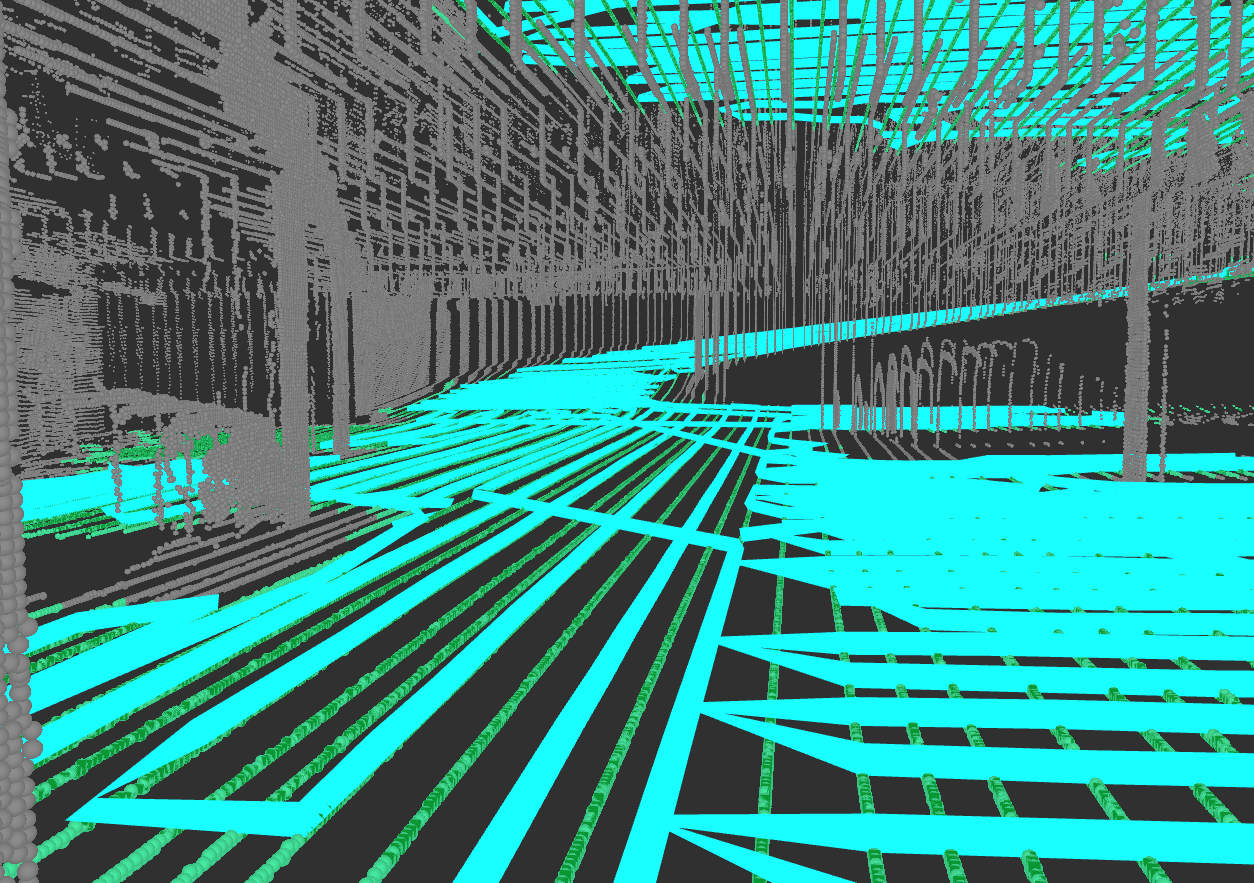
\includegraphics[width=\textwidth]{figures/garage_6.png}
		\end{subfigure}
		\begin{subfigure}{0.45\columnwidth}
			\centering
			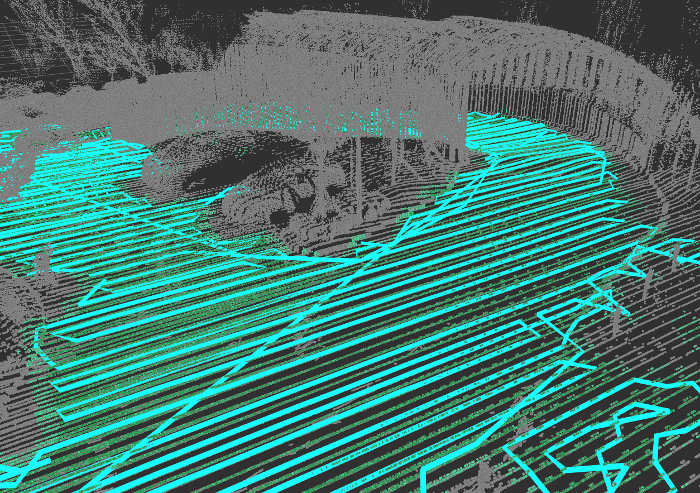
\includegraphics[width=\textwidth]{figures/garage_4.png}
		\end{subfigure}
		\\\vspace{0.35em}
		\begin{subfigure}{0.912\columnwidth}
			\centering
			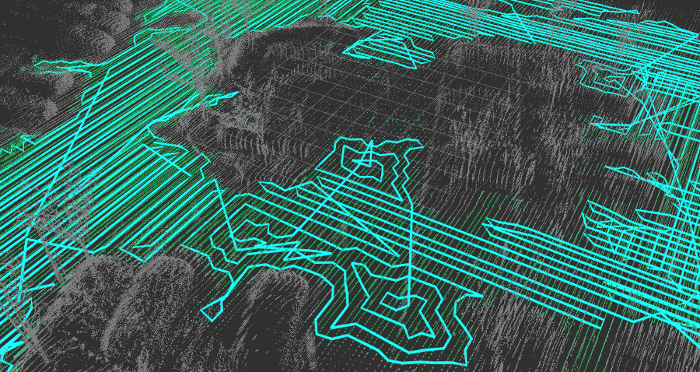
\includegraphics[width=\textwidth]{figures/garage_3.png}
		\end{subfigure}
		\caption{Two-storey Garage point cloud. Coverage path, our approach. Gray points are inaccessible and green points are traversable.}
		\label{fig:example}
	\end{figure}
	
	Real 3D environments are captured using LIDAR or 3D-sensors as point clouds. Further discretization can be made, for example using Octomap \cite{octomap}, but there are several benefits with working directly on a point cloud. Good coverage can be achieved while avoiding an intractably high voxel resolution, given that the point cloud distribution is fairly even over surfaces and that the point density is kept down to manageable levels. Furthermore, while planar or voxel-based surface approximations can be efficient representations, motion planning on such approximations may lead to unfeasible plans. A plan that seemed to be the shortest of all explored alternatives can be impossible to follow, lead to unsafe execution or be worse (e.g. take longer to follow) than other plans which seem worse during planning \cite{krusi2017driving}.
	%TODO: Also, motion planning on point clouds: \cite{krusi2017driving}. They have motivations, eh?
	
	The task investigated in this paper is that of CPP for autonomous road sweeping (Figure \ref{fig:example}), where the input is a point cloud and the output is a collision free path with highest possible coverage while minimizing path length and total rotation.
	%TODO (related work?): Previous work \cite{bormann2018indoor} (and their previous work) map indoor environment and has pipeline for automatic segmentation of map into single rooms and TSP for efficient visitation between rooms.	
	The main contributions of this paper are:
	\begin{itemize}
		\item A benchmark suite\footnote{Code and benchmark suite will be made available upon paper acceptance.} consisting of three large-scale urban environments as point clouds, with and without labeled points. They span a variety of multi-floor and complex geometry, representative of outdoor road sweeping tasks under difficult and varying real-world conditions.
		\item Evaluation of prominent CPP algorithms on the urban outdoor CPP task.
		\item A proposed CPP algorithm that out-performs state-of-the-art CPP algorithms at this task.
		\item Parameter optimization of CPP algorithms for automatic domain adaptation, for evaluation and as part of an enhanced offline meta-CPP algorithm.
	\end{itemize}
	
	The outline is as follows. In section \ref{sec:problem} the problem is formally summarized, in section \ref{sec:related-work} related work is discussed and relevant background material is presented in \ref{sec:background}. Section \ref{sec:terrain-assessment} describe how 3D point clouds are analyzed to determine the sets of points traversable and coverable by the robot. The proposed CPP algorithm is detailed in section \ref{sec:proposed-method}, and the benchmark suite including, three 3D point clouds representative for the urban road sweeping task, is presented in \ref{sec:scenario-environment}. Section \ref{sec:evaluation} contains the evaluation of CPP algorithms on the benchmark and section \ref{sec:conclusions} concludes the paper.
	
	\section{Problem Formulation}
	\label{sec:problem}
	%TODO: Heading angle (or full 6-DOF?)
	Consider a robot with geometry $R\subset \mathbb{R}^3$ that can travel over a surface with a maximum height difference of $h^R_{max}$.
	Given a bounded 3D world $\mathcal{W}\subset\mathbb{R}^3$ and a starting point $x_S$, the set $\mathcal{W}_{cov}\subseteq \mathcal{W}$ contains all surface points coverable by the robot. A surface point $p$ is coverable if there is a point $x\in\mathcal{W}$ for which the robot placed at $x$ cover $p$ with its geometry $R$, and if $x$ is reachable from $x_S$ without collisions.
	%TODO: The reachable points form the set W_\text{trav} of traversable point!
	
	The Coverage Path Planning (CPP) problem is to find a path $P$ of points $x\in P$ such that every point $p\in\mathcal{W}_{cov}$ must have been inside $R$ at least once when placing $R$ at every position in $P$. 
	The task here is to determine $\mathcal{W}_{cov}$ and subsequent a path starting in $x_S$ that let the robot cover all coverable points $x\in\mathcal{W}_{cov}$ while minimizing the path cost.
	
	\section{Related Work}
	\label{sec:related-work}
	Coverage path planning is still an open problem in robotics \cite{tan2021comprehensive}, with some of the issues being planning efficiency, path optimality, handling dynamic obstacles and dealing with complex environments. These issues are considered some of the major challenges in robotics, and CPP particularly challenging in complex and large-scale environments. For large-scale environments, offline CPP algorithms are the most common due to limitations on onboard hardware \cite{tan2021comprehensive}.
	
	%TODO: !!!!!!!!!!!!!!!!!
	%\textbf{TODO: } Discuss - Grid, cell, ??, point cloud representations - and outline how our work differs from the rest here.
	%Stoff: Our problem formulation differs from related work. The sets of traversable and coverable points are not the same set. We operate on a point cloud, not on a grid or explicit cells (although we have implicit cells?). We must determine which points (regions) that are traversable and coverable. The environment under consideration can be multi-floor but is outdoor (\cite{terrainassessment} is multi-floor terrain assessment in small confined indoor settings. Their related work is concerned with larger outdoor but single-floor terrain assessment. Note: old papers..).
	
	The development of robots for floor cleaning and road sweeping has a long history \cite{prassler2000short} and so does the development of algorithms for coverage path planning for robotics \cite{galceran2013survey}. Although the mechatronic and control development of road sweeping robots keep advancing \cite{rayguru2021output}, very little prior work \cite{chang2010design} exists on applying CPP to autonomous road sweeping and none that we can find in a realistic setting. One reason for the past dominance of CPP in the indoor setting \cite{galceran2013survey} can be due to the computational issues of scaling up current methods \cite{tan2021comprehensive}, not least grid- and cell-based methods \cite{miao2018scalable}, to the large scales of urban outdoor areas. Outdoor urban environments pose many challenges even to standard path planning \cite{krusi2017driving}, and thus also to coverage path planning.
	
	A recent survey \cite{bormann2018indoor} of CPP methods for indoor floor cleaning conclude after extensive empirical evaluations that Boustrophedon motion is the most prominent performer on covering single rooms. Multi-room single-floor apartments are separated into individual rooms covered in isolation. In \cite{miao2018scalable} they note that a major weakness of BA* \cite{choset1998coverage}, which apply Boustrophedon motion locally such as each room, is the long paths between the locally covered regions.
	
	The general poor performance of grid-based methods on large scale environments can be alleviated by rectangular decomposition as a pre-processing step \cite{miao2018scalable}, making the proposed method suitable for floor cleaning tasks in large scale environments such as a gym, library, warehouse or airports. They also consider cluttered indoor environments, e.g. gym equipment and library book shelves. The environment is, apart from these aspects, similar to the general characteristics in the indoor literature with a single rectangular room, simple and straight borders, and a planar and single floor.
	
	The geometry of non-planar surfaces can be taken into account to make the coverage path more energy efficient \cite{dogru2015towards}, for example by driving orthogonal to the slope. The drive direction can also affect the actual coverage achievable in cases where elevation is projected down onto a grid and solved using grid-based CPP methods \cite{hameed2016side}. By solving CPP in 3D instead, such as directly on the point cloud, such projection based issues are eliminated. Energy efficiency can be taken into consideration directly in the motion planning and it is straight forward to plan over multiple floors \cite{krusi2017driving}.
	
	%Large indoor environments (grid size of 4000x4000) are considered by \cite{miao2018scalable} such as a library, a gym, an airport. They show that BA* generates best local paths, but long paths between local regions. They propose a method that is better than BA* on the total path length. Seem to generate more rotations though..? (We might need to motivate why we didn't compare with their proposed approach)
	
	\section{Background}
	\label{sec:background}
	Coverage path planning algorithms relevant for understanding the proposed algorithm are described here, followed by the parameter optimization technique utilized in this work.
	
	The CPP algorithms BA* \cite{viet2013ba} and Inward Spiral \cite{zhang2019path} are representative of a family of methods which are well performing in a variety of settings. The proposed algorithm (\ref{sec:proposed-method}) combine ideas from these. An overview of the algorithms are presented here, for more details see the references.
	
	\subsection{CPP algorithm: BA*}
	BA* \cite{viet2013ba} is based on Boustrephedon motions \cite{choset1998coverage}, which are a kind of zigzag motion. The idea is to cover a local regions with a zigzag pattern, then find the shortest path to the next uncovered position and repeat the behavior until completeness. The algorithm consists of the following steps:
	\begin{enumerate}
		\item Cover the local area using the Boustrophedon motion (BM) algorithm until a critical point is reached and no further Boustrophedon motion is possible.
		\item Use a backtracking list to find the next starting point.
		\item Use A* \cite{russell_artificial_2020} to plan a collision free path to the next starting point.
		\item Shorten the path using the A*SPT \cite{viet2013ba} algorithm.
		\item Follow the path and go to step 1 to cover a new area.
	\end{enumerate}
	These steps are repeated until Step 2 can no longer find a new uncovered starting point.
	
	\subsection{CPP algorithm: Inward Spiral}
	Inward Spiral \cite{zhang2019path} works by counter-clockwise motion. The algoritm consists of the following steps:
	\begin{enumerate}
		\item Clean area in an inward spiral motion until a dead zone
		\item Find closest uncovered accessible point using Breadth-first search \cite{russell_artificial_2020}.
		\item Find shortest path using A* to the closest uncovered point and go back to Step 1.
	\end{enumerate}
	This cycle repeats until the area has been covered.
	
	\subsection{Parameter Optimization}
	\label{sec:parameter-optimization}
	Bayesian Optimization (BO) \cite{shahriari2015taking} is a gradient-free optimization method powered by probabilistic inference, where the uncertainty of the objective function is modelled across the input range. It is a sequential process: The next input to evaluate is the most likely input candidate to produce the lowest expected loss given all previously investigated inputs so far. BO is much more sample efficient than other types of optimization methods. It is well suited for situations where it is costly to try a new input value, which makes it important to try out as few as possible while still having a reasonably high probability of finding a global minimum.
	
	HyperOpt \cite{bergstra2013making} is a widely used parameter optimization library implementing Bayesian Optimization. It is most often used for parameter tuning in machine learning, but the applicability of BO is widespread \cite{shahriari2015taking}  and in this work it is used as an automatic method to adapt the CPP algorithms to the specific domain. Tedious and ad hoc hand tuning is replaced with a systematic and automatic modern method.
	
	\section{Terrain Assessment}
	\label{sec:terrain-assessment}
	%	\textbf{TODO: } Add reference to some robot that is supposed to move through the terrain (it has some geometry and a max-step..constant), otherwise we do not know how to distinguish Accessible (traversable) and Coverable.
	%	
	\begin{figure}[t]
		\centering
		\begin{subfigure}{.49\columnwidth}
			\centering
			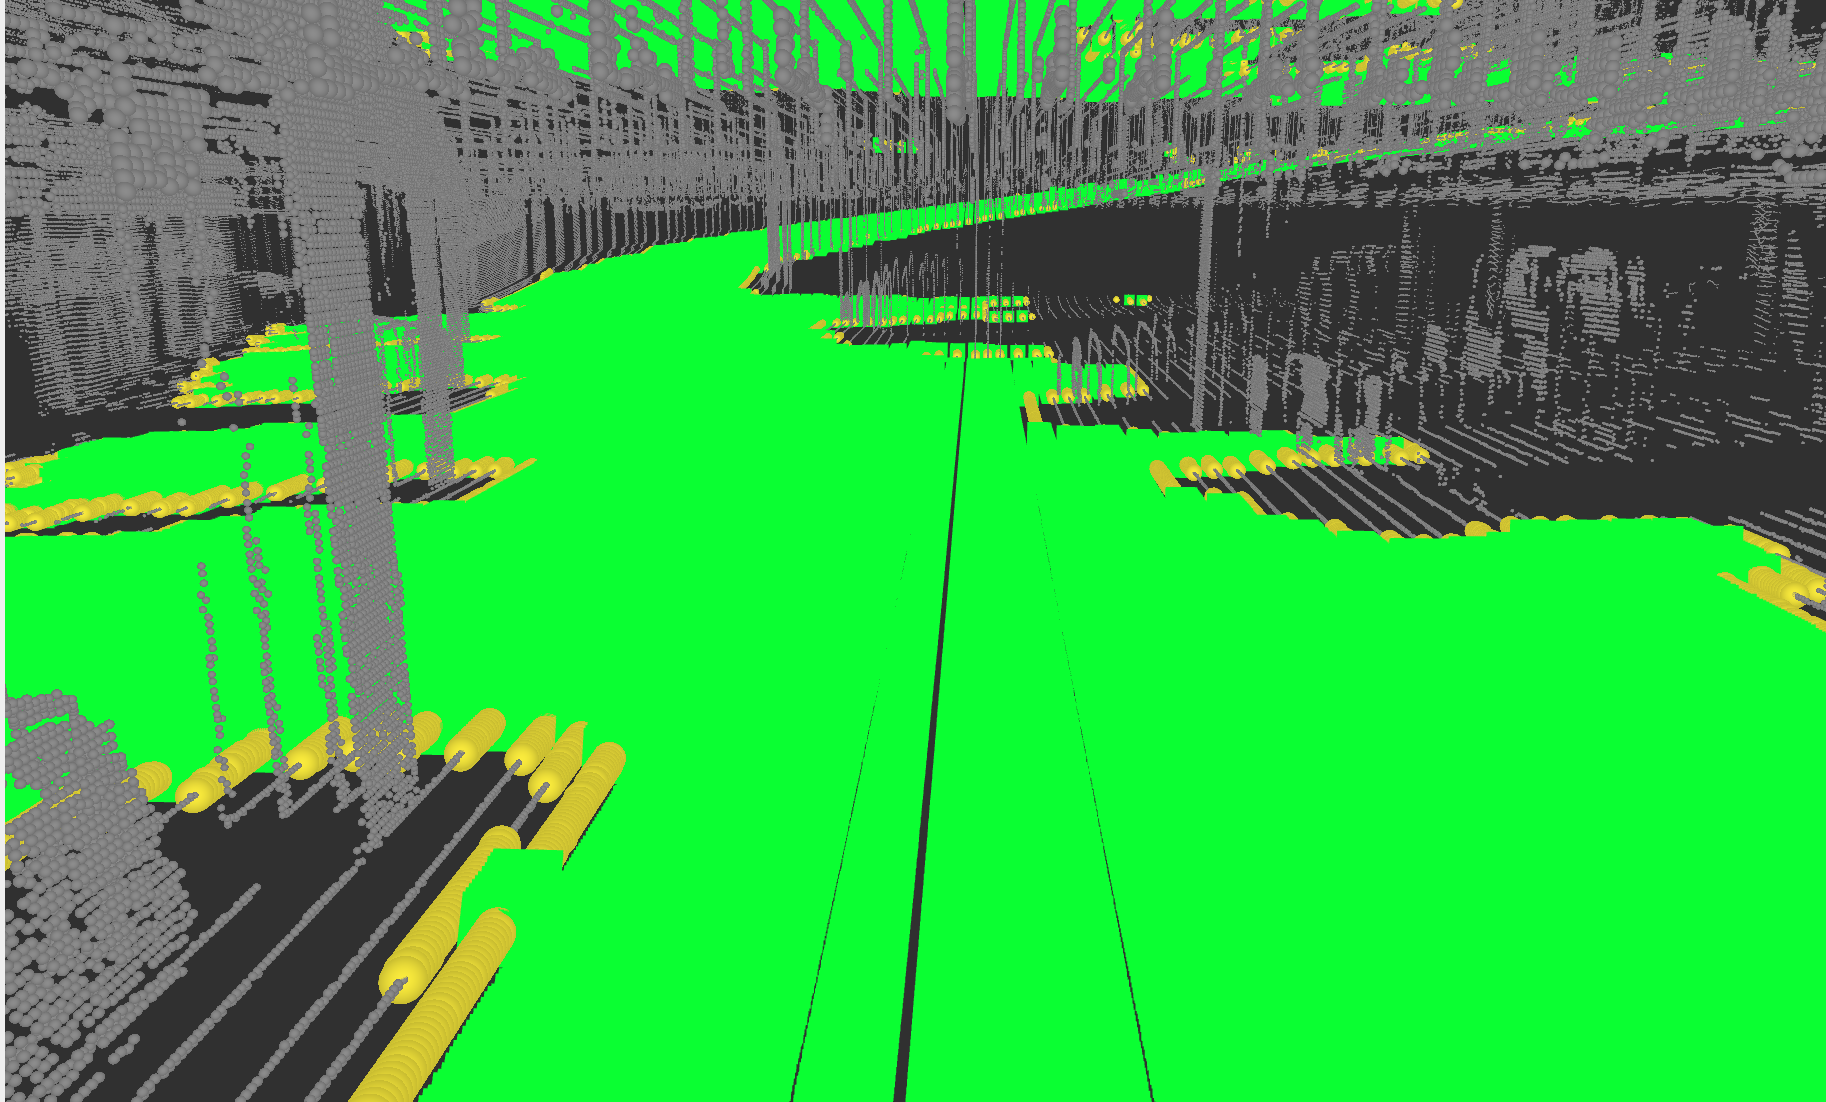
\includegraphics[width=\textwidth]{figures/terrainassessment-floor1.png}
			\caption{View of floor 1.}
		\end{subfigure}
		\begin{subfigure}{.49\columnwidth}
			\centering
			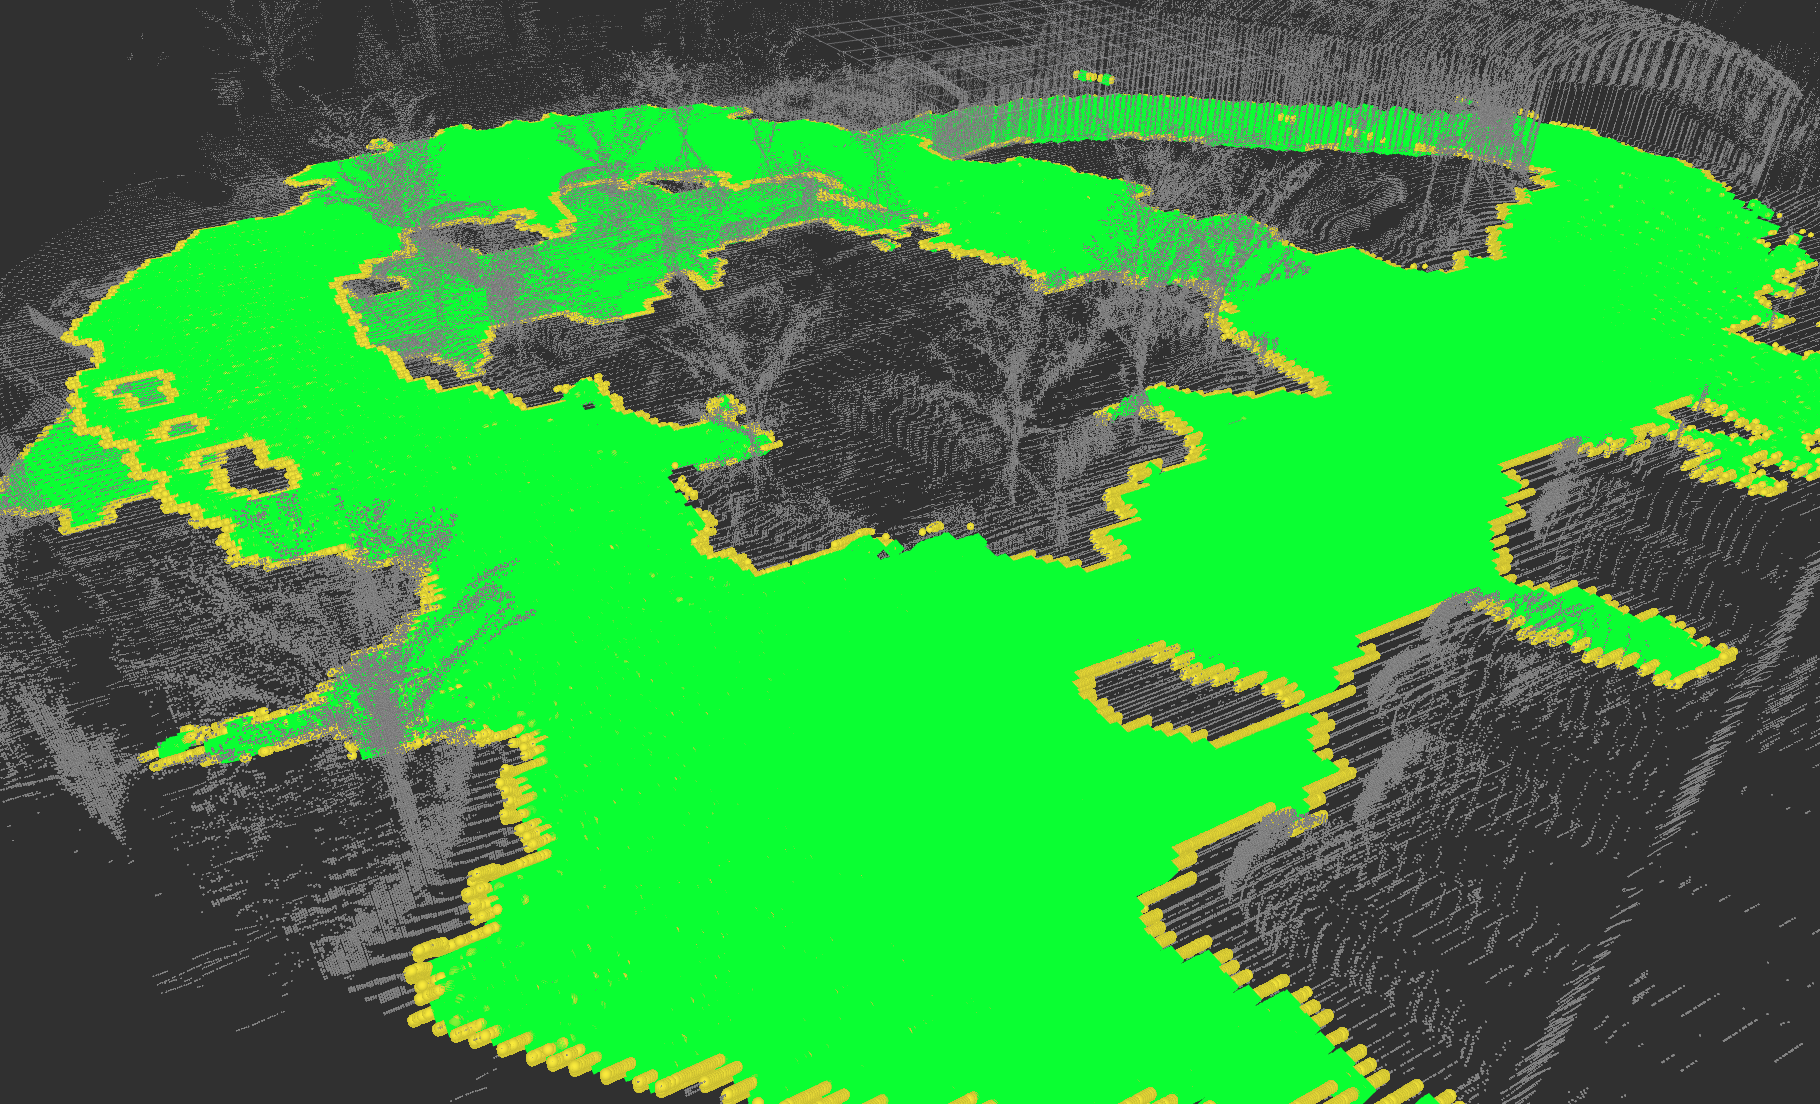
\includegraphics[width=\textwidth]{figures/terrainassessment-floor2.png}
			\caption{View of floor 2.}		
		\end{subfigure}	
		\caption{Terrain Assessment of the Two-storey Garage point cloud. Green points represent traversable areas, yellow are non-traversable but coverable and grey points are inaccessible.}
		\label{fig:terrainassessment-example}
	\end{figure}
	To navigate a robot in a an environment, knowledge about traversable positions is required. As in \cite{krusi2017driving} we chose to keep the terrain representation \emph{continuous} and move between 3D positions. Since we do both motion planning and covering, coverable positions also needs to be known. See Figure~\ref{fig:terrainassessment-example} for examples. To guarantee that traversable and coverable positions are drivable they are restricted to classified points. 
	
	The purpose of the terrain assessment is to classify points in a given point cloud. Points are classified as:
	\begin{itemize}
		\item \textbf{Inaccessible} - Can not overlap with robot geometry.  
		\item \textbf{Traversable} - Can be visited by the robot without collision with an obstacle.
		\item \textbf{Coverable} - Can be covered by the range of the robot after visiting every traversable point.
	\end{itemize}
	
	Our method is based on robot specific properties such as robot height, maximum navigable step height, covering range and robot breadth. The covering range and the breadth are assumed to be the same and defined by a radius from current position of the robot.
	\begin{enumerate}
		\item \textbf{Floor segmentation} - Divide the point cloud into different floors by splitting the points into vertically stacked layers and finding heights with the largest amount of points as in \cite{terrainassessment}.
		\item \textbf{Cell segmentation} - For each floor separately. Create a Digital Elevation Model (DEM) of the floor by splitting the point cloud into cells and finding the elevation using the method in \cite{terrainassessment}. It looks for free space between two points in a cell larger than the robot height. If found, the elevation is set to the lowest point.
		\item \textbf{Cell classification} - A Breadth First Search is then used to find the biggest connected area of coverable cells. The DEM is used to prevent steps where the height difference between cells is too big.
		\item \textbf{Point Classification} - Classify points with these steps: 
		\begin{enumerate}
			\item Set all points that are not in the main coverable area as \emph{Inaccessible}
			\item Set all points in the main coverable area that are more than a robot radius away from an \emph{Inaccessible} point as \emph{Traversable}.
			\item Set all points that are within a robot radius from a \emph{Traversable} point as \emph{Coverable}.
		\end{enumerate}
	\end{enumerate}
	
	This method does not guarantee that every traversable point is accessible from the main coverable area. Step 4b) makes narrow passages nontraversable which separates clusters of points from the main coverable area and consequently, make 100\% coverage unreachable. 
	%To get knowledge about the actual reachable coverage a breadth first method \cite{russell_artificial_2020} with parameter optimization \cite{bergstra2013making} over step size and visited threshold (\ref{sec:CPP-point-cloud}) over cost function $c~=~1~-~coverage$. 
	%%Two parameters is optimized with the cost function $c = 1 - coverage$. 
	%%\begin{itemize}
	%%    \item \textbf{Step size} - Length of the step taken in 8 different directions at each step.
	%%    \item \textbf{Visited threshold} - Minimum distance from a position to a previously visited points to be classified as visited.   
	%%\end{itemize}
	%The actual reachable coverage is given by the lowest cost that were reached when using the optimised parameter values. 
	
	\subsection{CPP on a Point Cloud}
	\label{sec:CPP-point-cloud}
	The CPP methods in Section \ref{sec:background} are designed for operation on a grid or cell-network. To work on a point cloud it is necessary to define how valid steps, from one traversable point to another, is done. In this work we use 8-connectivity on the point cloud manifold. Each CPP algorithm have a step size $\lambda_{CPP}$ and a visited distance-threshold $r_{visited}$ 
	%(Table \ref{tab:cpp_parameters}) 
	which control valid expansions of the algorithms. Given a traversable point, a neighbour point is found in either direction by selecting the closest traversable point $\lambda_{CPP}$ away in the specific direction. The neighbour is already visited if a previously expanded traversable point is within a $r_{visited}$ distance of the neighbour.
	%	\begin{table}[h!]
	%		\centering
	%		\caption{General CPP parameters and descriptions.}
	%		\begin{tabular}{|l|c|}
	%			\hline 
	%			\textbf{Parameter} & \textbf{Description}\\
	%			\hline 
	%			$\lambda_{CPP}$ & Step size in CPP algoithms\\
	%			$r_{visited}$ & Threshold for a point to be visited\\
	%			\hline 
	%		\end{tabular}	
	%		\label{tab:cpp_parameters}
	%	\end{table}
	
	%	\textbf{TODO: } BFS from a starting point (could have been anywhere in the traversable space) to calculate actual possible coverage using the robot geometry moving in the point cloud. Describe the process of optimizing the two relevant parameters (step-size and visited-threshold) and why this is done.
	%	\textbf{Fr�ga: } Hur refererar man till ett steg som ovan (4b))
	%	\textbf{Fr�ga: } Beh�ver man referera till BFS?
	
	\begin{algorithm}
		\small
		\SetAlgoLined
		\KwData{Starting position $p_s$. $W = \emptyset$}
		\KwResult{Path $W$ to cover the area.}
		%$S = \emptyset$\\
		$S_\text{BA*} \gets \text{Sample BA* (Algorithm \ref{alg:myalgorithm_sample_BAstar})}$  \\
		$S_\text{IS} \gets \text{Sample Inward Spiral (Algorithm \ref{alg:myalgorithm_sample_Inward_Spiral})}$  \\
		$S \gets S_\text{BA*} \cup S_\text{IS}$\\
		%		\While{\textup{Coverage $C_1$ or iteration $N^{iter}_{max}$ has not been reached}}{
		%			$p_r$ = \textup{random uncovered point}\\
		%			$S_{BA*} = \emptyset$\\
		%			\For{\textup{angle $\phi \in [0,1, ..., N_{\phi}] \cdot 2\pi/N_{\phi} $ }}{
		%				\textup{Set $W_{BA*} \rightarrow$ Generated BA* path with north being towards angle $\phi$ starting at $p_r$}\\
		%				$S_{BA*} = S_{BA*} \cup W_{BA*}$\\
		%			}
		%			$W_{best}$ = \textup{Path $W_{BA*}$ in $S_{BA*}$ with the highest coverage} \\
		%			\If{\textup{Coverage of $W_{best} > C_{min}$}}{
		%				$S = S \cup W_{best}$  \\
		%			}
		%		}
		%		\While{\textup{Coverage $C_2$ has not been reached}}{
		%			$p_r$ = \textup{random uncovered point}\\
		%			\textup{Set $W_{Spiral} \rightarrow$ Generated Inward Spiral path with starting at $p_r$}\\
		%			\If{\textup{length of $W_{Spiral} > N_{min}$}}{
		%				$S = S \cup W_{Spiral}$  \\
		%			}
		%		}
		$T \gets$ \textup{Empty graph tree}\\
		\For{\textup{path $W_i$ in $S$}}{
			\textup{Add start and end point of $W_i$ as nodes in $T$.}
		}
		$W_\text{TSP} \gets$ \textup{Cheapest route to visit all nodes in $T$}\\
		$p_{curr} \gets p_s$ \\
		$S_\text{TSP} \gets \emptyset$ \\
		\For{\textup{node $p_i$ in $W_\text{TSP}$}}{
			\If{$p_{i} = p_{curr}$}{
				\textup{\textbf{continue}}
			}
			\eIf{\textup{$p_i$ is a start node}}{
				$W_i \gets $\textup{ Path in $S$ with $p_i$ as start node} \\
			}{
				$W_i \gets $\textup{ Reversed path in $S$ with $p_i$ as end node} \\
			}
			$S_\text{TSP}.\texttt{push\_back}(W_i)$ \\
			$p_{curr} \gets \text{Last point in }W_i$ \\
		}
		$p_{curr} \gets p_s$ \\
		\For{\textup{path $W_i$ in $S_\text{TSP}$}}{
			$W_{A*} \gets$ Shortest path from $p_{curr}$ to the start point of $W_i$. \\
			$W \gets W \cup {W_{A*}, W_i}$ \\
			$p_{curr} \gets \text{Last point in }W_i$ \\
		}
		\textup{\textbf{return $W$}}
		\caption{Sample Based BA* \& Inward Spiral.}
		\label{alg:myalgorithm}
	\end{algorithm}
	%
	\begin{algorithm}
		\small
		\SetAlgoLined
		\KwData{$S = \emptyset$}
		\KwResult{Set of paths $S$ covering local regions.}
		\While{\textup{Exploration $E^1$ has not been reached}}{
			$s_r$ = \textup{random position in uncovered area}\\
			$p_r$ = \textup{closest border point to $s_r$ given by BFS}\\
			$S_{BA*} = \emptyset$\\
			\For{\textup{angle $\phi \in [0,1, ..., N_{\phi}] \cdot 2\pi/N_{\phi} $ }}{
				$p_s \gets p_r$ \\
				\While{$\text{distance to} p_s < d^1_{max}$}{
					$W_{BA*} \gets \text{BA* at } p_s \text{ with north } = \phi $\\
					$p_s \gets \textup{new starting point in backtracking list}$ \\
				}
				$S_{BA*} = S_{BA*} \cup W_{BA*}$\\
			}
			$S_{BA*_{accepted}} \gets W_{BA*} \text{with } \frac{\text{cost}}{\text{coverage}} > C^1_{min}$\\
			\eIf{$S_{{BA*}_{accepted}} = \emptyset$}{
				$W_{best} \gets W_{BA*} \in S_{BA*} \text{with max coverage}$ \\
			}{
				$W_{best} \gets W_{BA*} \in S_{BA*} \text{with lowest } \frac{\text cost}{\text coverage}$ \\
				$S = S \cup W_{best}$ 
			}
			$E^1 \gets \text{covered points by} W_{best}$ \\
			
		}
		\textup{\textbf{return $S$}}
		\caption{PART I: Sample BA*}
		\label{alg:myalgorithm_sample_BAstar}
	\end{algorithm}
	%
	\begin{algorithm}
		\small
		\SetAlgoLined
		\KwData{$S \gets \emptyset$}
		\KwResult{Set of paths $S$ covering local regions.}
		\While{\textup{Goal coverage $C$ has not been reached}}{
			$s_r$ = \textup{random position in uncovered area}\\
			$p_r$ = \textup{closest border point to $s_r$ given by BFS}\\
			$p_s \gets p_r$ \\
			\While{$\text{distance to} p_s < d^2_{max}$}{
				$W_{Spiral} \gets \text{Inward Spiral at } p_s$
				$p_s \gets \textup{new starting point using BFS}$ \\
			}
			\If{$\frac{\text{cost}}{\text{coverage}} \text{ of } W_{Spiral} > C^2_{min}$}{
				$S \gets S \cup W_{Spiral}$  \\
			}
		}
		\textup{\textbf{return $S$}}
		\caption{PART II: Sample Inward Spiral}
		\label{alg:myalgorithm_sample_Inward_Spiral}
	\end{algorithm}
	
	\section{Proposed Method\\(Sampled BA* \& Inward Spiral)}
	\label{sec:proposed-method}
	
	%\begin{algorithm}
	%	\SetAlgoLined
	%	\KwData{Starting position $p_s$, Coverage percentage goals $C_1$ and $C_2$}
	%	\KwResult{Path $W$ to cover the area.}
	%	
	%	\textup{\textbf{return $W$}}
	%	\caption{Sample Based BA* and Inward Spiral with Traveling Salesman.}
	%	\label{alg:myalgorithm}
	%\end{algorithm}
	
	\begin{table}[t]
		\centering
		\caption{Sampled BA* \& Inward Spiral parameters.}
		\begin{tabular}{|l|l|c|}
			\hline 
			\textbf{Parameter} & \textbf{Description} \\
			\hline 
			$E^1$ & Exploration goal for PART I \\
			$C$ & Total coverage goal\\
			$d^1_{max}$ & Max distance to next starting point in PART I\\
			$d^2_{max}$ & Max distance to next starting point in PART II\\
			$C^{1}_{min}$ & Min cost (length + rotation) per coverage in PART I \\
			$C^{2}_{min}$ & Min cost (length + rotation) per coverage in PART II \\
			$\lambda_{CPP}$ & Step size\\
			$r_{visited}$ & Visited threshold\\
			\hline 
		\end{tabular}	
		\label{tab:sampled_parameters}
	\end{table}
	
	\begin{figure*}[!b]
		\centering
		\begin{subfigure}{0.29\textwidth}
			\centering
			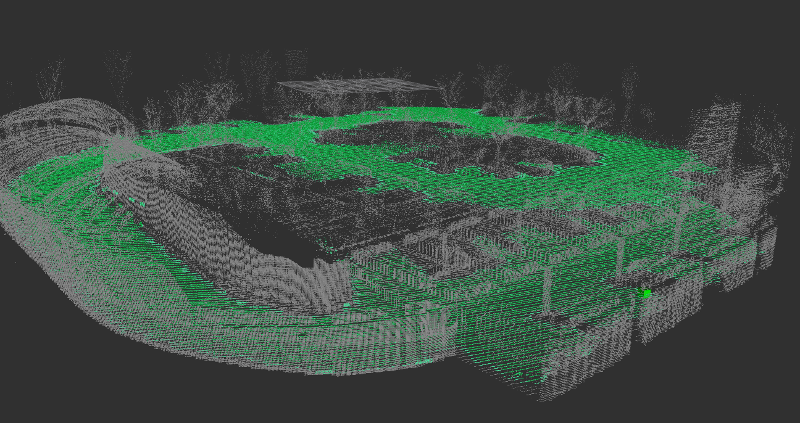
\includegraphics[width=\textwidth]{figures/garage_terrain.png}
			\caption{Two-storey Garage}
			\label{fig:map_garage}
		\end{subfigure}
		\begin{subfigure}{0.29\textwidth}
			\centering
			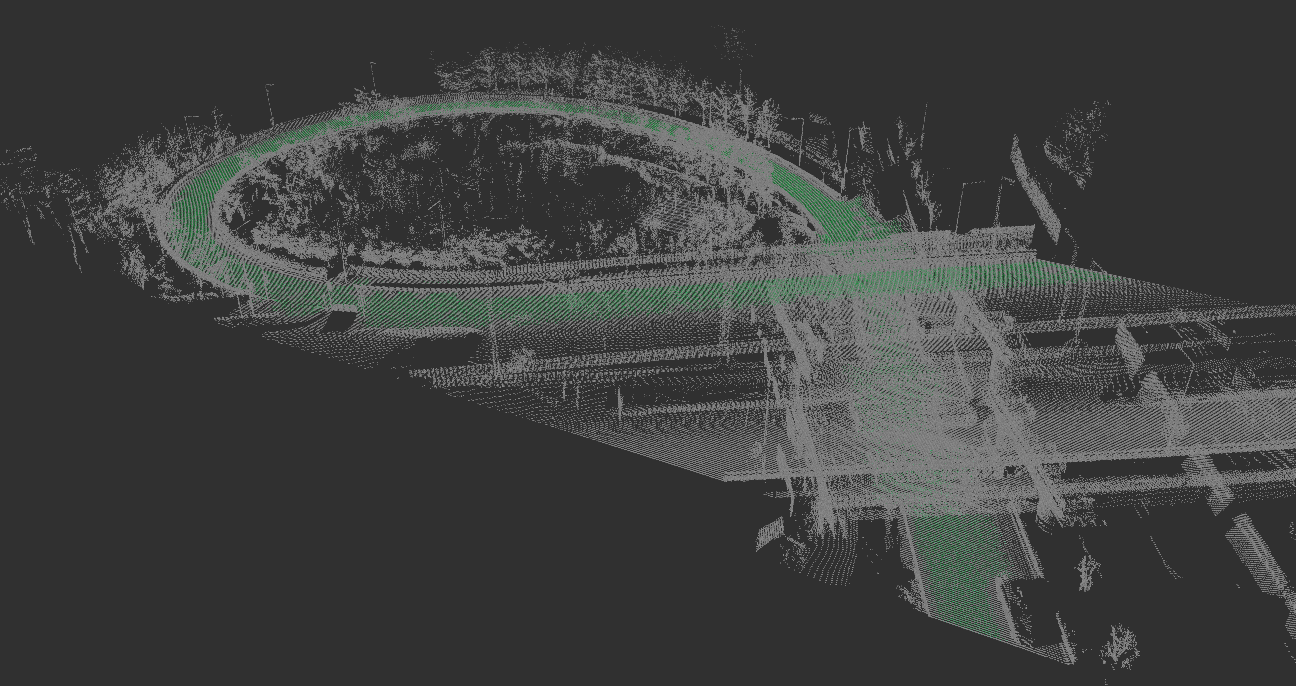
\includegraphics[width=\textwidth]{figures/map_bridge.png}
			\caption{Highway Bridge}
			\label{fig:map_highway}
		\end{subfigure}
		\begin{subfigure}{0.29\textwidth}
			\centering
			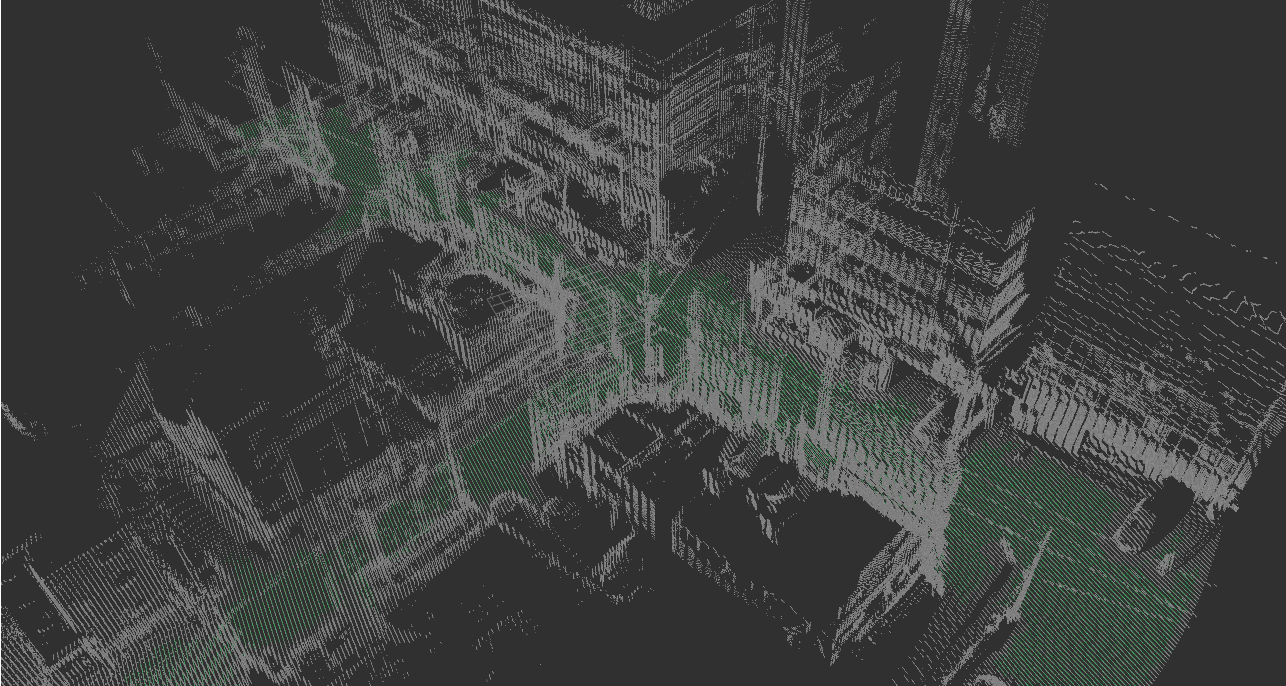
\includegraphics[width=\textwidth]{figures/crossing.png}
			\caption{City Crossing}
			\label{fig:map_crossing}
		\end{subfigure}
		\caption{}
		%\caption{Three complex outdoor environments.}
		\label{fig:maps}
		\begin{subfigure}{0.31\textwidth}
			\centering
			\includegraphics[width=\textwidth]{figures/results_garage.png}
			\caption{Two-storey Garage}
			\label{fig:result-garage-cost-coverage}
		\end{subfigure}
		\begin{subfigure}{0.31\textwidth}
			\centering
			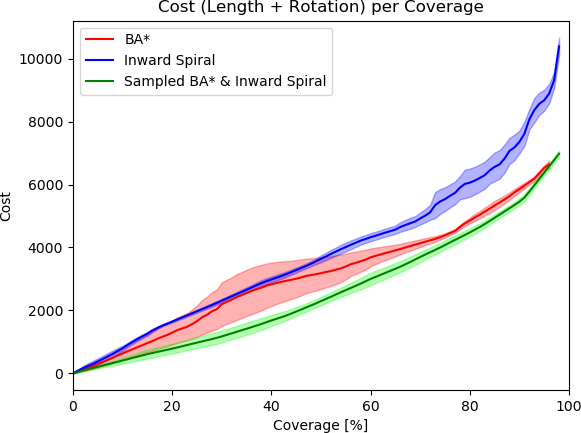
\includegraphics[width=\textwidth]{figures/results_bridge.png}
			\caption{Highway Bridge}
			\label{fig:result-bridge-cost-coverage}
		\end{subfigure}
		\begin{subfigure}{0.31\textwidth}
			\centering
			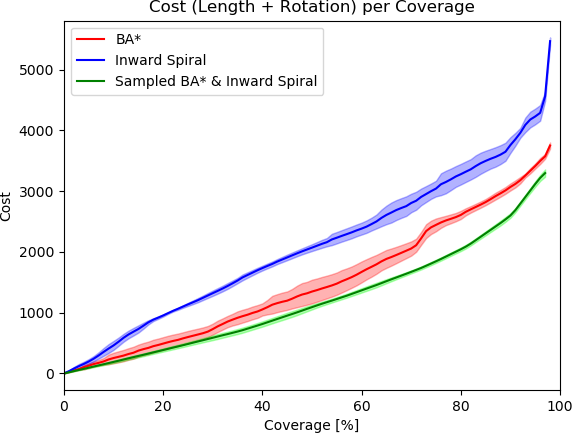
\includegraphics[width=\textwidth]{figures/results_crossing.png}
			\caption{City Crossing}
			\label{fig:result-crossing-cost-coverage}
		\end{subfigure}
		\caption{Performance results on the benchmark suite. Mean and 95\% confidence interval over 10 random staring locations.}
		\label{fig:result-cost-coverage}
		\begin{subfigure}{0.29\textwidth}
			\centering
			\centering
			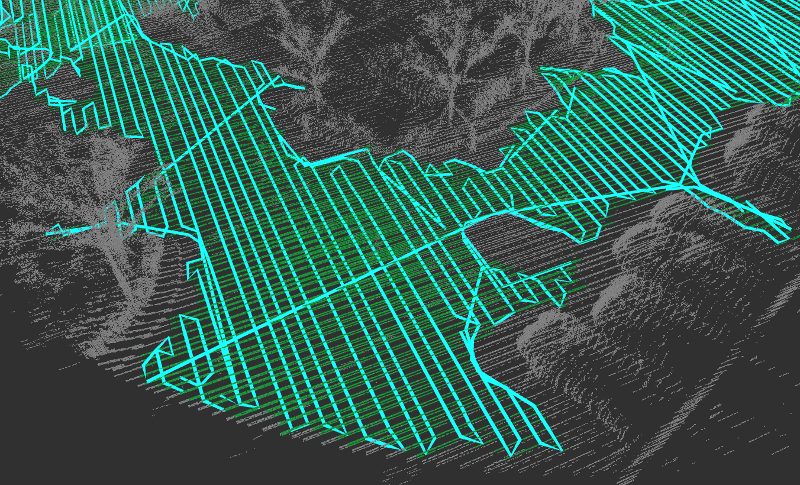
\includegraphics[width=\textwidth]{figures/example_bastar2.png}
			\caption{BA*}
			\label{fig:example_bstar}
		\end{subfigure}
		\begin{subfigure}{0.29\textwidth}
			\centering
			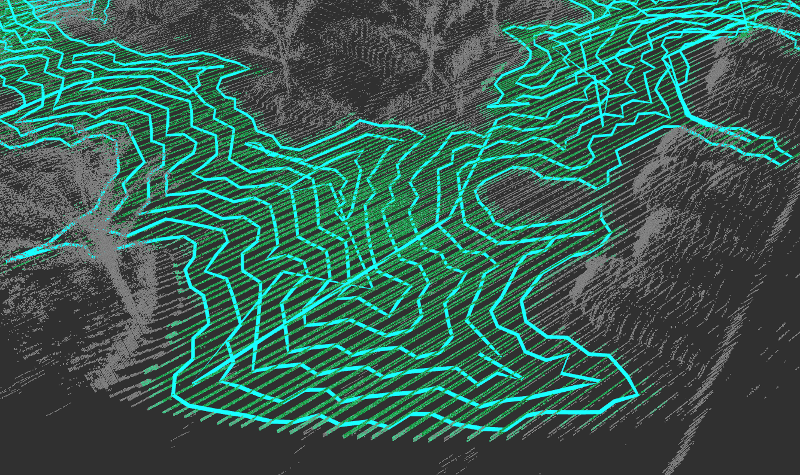
\includegraphics[width=\textwidth]{figures/example_inward_spiral.png}
			\caption{Inward Spiral}
			\label{fig:example_inward_spiral}
		\end{subfigure}
		\begin{subfigure}{0.29\textwidth}
			\centering
			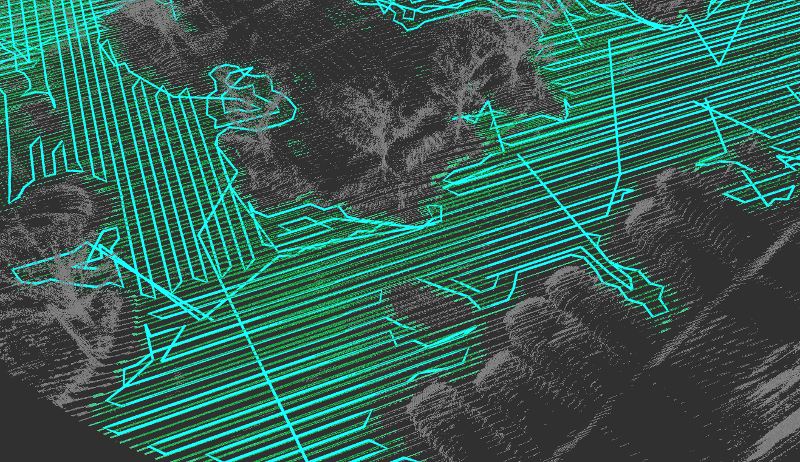
\includegraphics[width=\textwidth]{figures/example_new_sampled.png}
			\caption{Sampled BA* \& Inwards Spiral}
			\label{fig:example_sampled_bstar}
		\end{subfigure}
		\caption{Coverage paths on the Garage environment. }
		\label{fig:algorithm_experiment_examples}
	\end{figure*}
	
	We propose a new CPP method, \textit{Sampled BA* \& Inward Spiral}, which combines the strengths of BA* \cite{viet2013ba} and Inward Spiral \cite{zhang2019path}, with inspiration taken from Sampling-Based Sweep Planning \cite{englot2012sampling}.
	The idea is to minimise the cost, defined as length + rotation, by covering open areas with BA* and more complex areas with Inward Spiral. This is done by covering segments of the area with BA* and Inward Spiral starting from random sampled points and then connect these segments with a TSP solver.
	%TODO: Is A* used to calculate cost of shortest path between each area, over which a TSP solver is used to determine visitation order?
	Sampled BA* \& Inward Spiral (Algorithm \ref{alg:myalgorithm}) consists of the following steps:
	\begin{enumerate}
		\item Initialise a list of segments $S$, covered points $P_{cov}$ and explored points $P_{exp}$.
		\item For $N_\phi = 4$ different angles $\phi_i$, define $north$ as the angle $\phi_i$ and start covering using the BA* algorithm \cite{viet2013ba} starting from a \emph{Traversable} border point of a randomly sampled uncovered area. Stop covering when the distance to the next starting point in the backtracking list exceeds $d^1_{max}$. 
		\item If no path had a cost per coverage that were lower than $C^{1}_{min}$, choose the path with the biggest coverage and add all covered points by the chosen path to $P_{exp}$.  Otherwise, choose the path with the lowest cost per coverage. Add it to $S$ and add points that were covered by it to $P_{cov}$ and $P_{exp}$.
		\item Repeat Step 2-3 until the exploration percent, given by the size of $P_{exp}$, reaches $E^1$.
		\item Start covering using the Inward Spiral algorithm \cite{zhang2019path} starting from a \emph{Traversable} border point of a randomly sampled uncovered area. Stop covering when the distance to the next starting point exceeds $d^2_{max}$. If cost per coverage is lower than $C^{2}_{min}$, add path to $S$.
		\item Repeat the Step 5-6 until $P_{cov}$ gives coverage $>C$.
		\item Repeat Step 5-6 until the exploration percent, given by the size of $P_{exp}$, reaches $E^1$.
		\item Construct a graph tree, $T$, from $S$. Only the start and end positions of the paths in $S$ are added as nodes to $T$. All nodes are connected with edges with weights% set to 
		\begin{itemize}
			\item $w=0$, if the edge is between the start and end node of the same path in $S$.
			\item Otherwise, distance based  according to equation 
			\begin{align}
			\label{eq:distanebased}
			w = \;&w_\text{offset} + 
			| s_A(x,y) - s_B(x,y) | +\nonumber\\
			&K | s_A(z) - s_B(z) |\nonumber
			\end{align}
			where $s_A$ and $s_B$ are the position of the two nodes, $w_\text{offset}$ is a large number and $K\geq 1$.
		\end{itemize}
		The purpose of $w_\text{offset}$ is to make sure that the traveling salesman algorithm in the following step always chooses to connect corresponding start and end nodes. Since the environment could have multiple floors, extra weight $K$ is added to difference in height, to avoid potential movement between floors.  
		\item Solve the TSP problem \cite{python-tsp} of the cheapest visitation order, $W_\text{TSP}$, to visit all nodes in $T$.
		\item Walk through every node in $W_\text{TSP}$ and create an ordered list of paths $S_\text{TSP}$. For every node $s_i$,
		\begin{itemize}
			\item If $s_i$ is start node, add corresponding path %in $S$ 
			to $S_\text{TSP}$.
			\item If $s_i$ is a end node, add the corresponding path, but reversed, in $S$ to $S_\text{TSP}$.
		\end{itemize}
		\item Create a continuous path $W$ by following the paths in $S_\text{TSP}$. Connect them with obstacle free smooth paths.
	\end{enumerate}
	
	The algorithm parameters are listed in Table \ref{tab:sampled_parameters}.
	
	\section{Autonomous Road Sweeping}
	\label{sec:scenario-environment}
	Road sweeping is a challenging task due to a complex environment, where the environment is somewhat unbounded and may have rough terrain \cite{chang2010design}. A particular difficulty of contemporary CPP algorithms is that of large-scale environments \cite{tan2021comprehensive}, even with simple geometry. We consider the challenging task of a road sweeping robot in an urban setting, where offline CPP is sufficient but where CPP is performed on a large-scale map with complex geometry. The benchmark suite consists of three environments (\ref{sec:benchmark-environments}) which are realistically represented as point clouds, collected from real urban environments. Part of the suite is also a scenario description (\ref{sec:benchmark-scenario}) which include specifications of a road sweeping robot, providing the necessary details to perform terrain assessment (\ref{sec:terrain-assessment}) and to evaluate CPP algorithms on the benchmark environments.
	%in a realistic simulation.
	
	
	\subsection{3D Environments}	
	\label{sec:benchmark-environments}
	%TODO
	%	\begin{itemize}
	%		\item 3 large-scale urban environments
	%		\item Their different stats and challenges
	%		\item Figures showing the environments and possibly traversable/coverable points in them, as well as the starting point?
	%	\end{itemize}
	%
	The three urban environments (Figure \ref{fig:maps}) consists of 3D point clouds that have been carefully selected from the large Complex Urban Dataset \cite{jjeong-2019-ijrr}. These environments represent different difficult, but typical, urban outdoor scenes. 
	
	The \emph{Two-storey Garage} environment consists of a parking lot with an underground garage right below. The point cloud is a subset of \textit{urban05} \cite{jjeong-2019-ijrr}. The main challenges are complex border geometry, multi-level aspect and the transition between levels. It contains $2.6$M points and has a total traversable area for the road sweeping robot of 1678m$^2$.
	The \emph{Highway Bridge} environment is a subset of \textit{urban17}, contains $2.3$M points and has a total traversable area for the road sweeping robot of 2637m$^2$. The main challenges are the very long curved drive-way together with its multi-level aspect.
	The \emph{City Crossing} environment is a subset of \textit{urban02}, contains $3.2$M points and has a total traversable area for the road sweeping robot of 1296m$^2$. The main challenge is the clutter and complex surface/border geometry.
	
	
	
	%	\begin{figure*}
	%		\centering
	%		\begin{subfigure}{0.46\textwidth}
	%			\centering
	%			
\includegraphics[width=\textwidth]{figures/map_garage.png}
	%			%\caption{Garage. Ground floor and basement floor.}
	%			\label{fig:map_garage}
	%		\end{subfigure}
	%		\begin{subfigure}{0.46\textwidth}
	%			\centering
	%			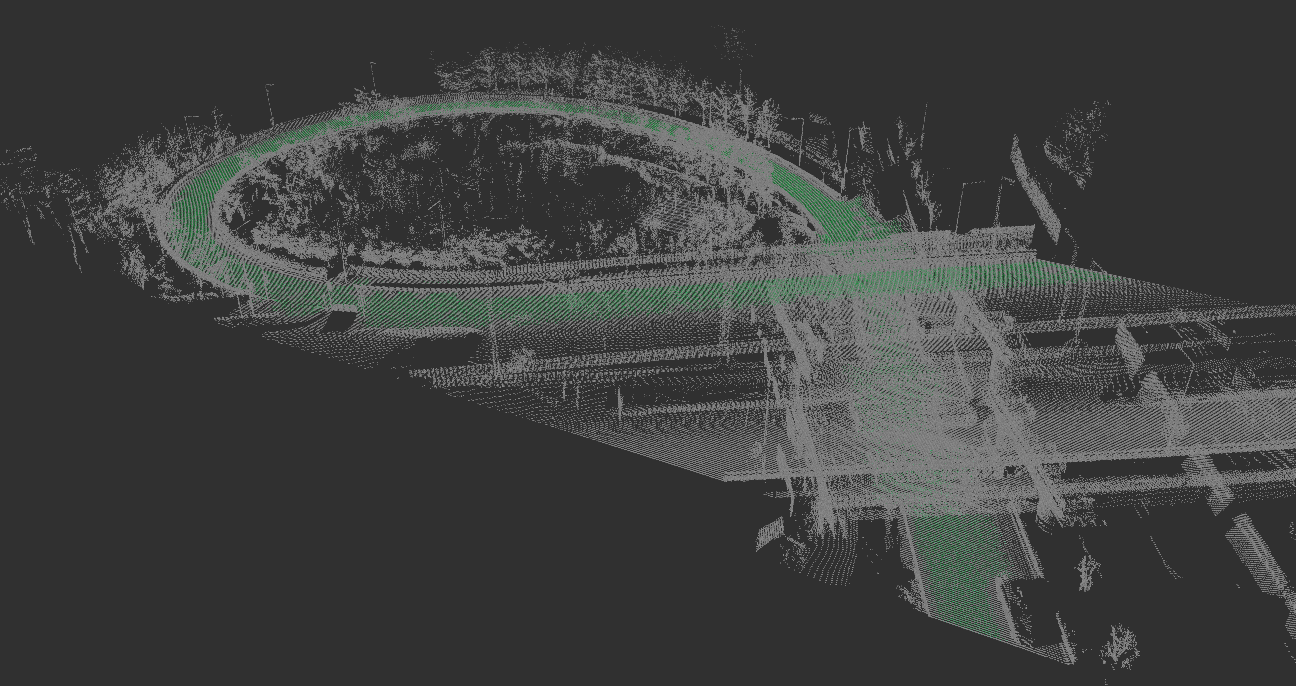
\includegraphics[width=\textwidth]{figures/map_bridge.png}
	%			%\caption{Highway. Bridge with XY-overlap.}
	%			\label{fig:map_highway}
	%		\end{subfigure}
	%		\\\vspace{-0.9em}
	%		\begin{subfigure}{0.46\textwidth}
	%			\centering
	%			
\includegraphics[width=\textwidth]{figures/map_crossing.png}
	%			%\caption{Crossing. Cluttered.}
	%			\label{fig:map_crossing}
	%		\end{subfigure}
	%		\begin{subfigure}{0.46\textwidth}
	%			\centering
	%			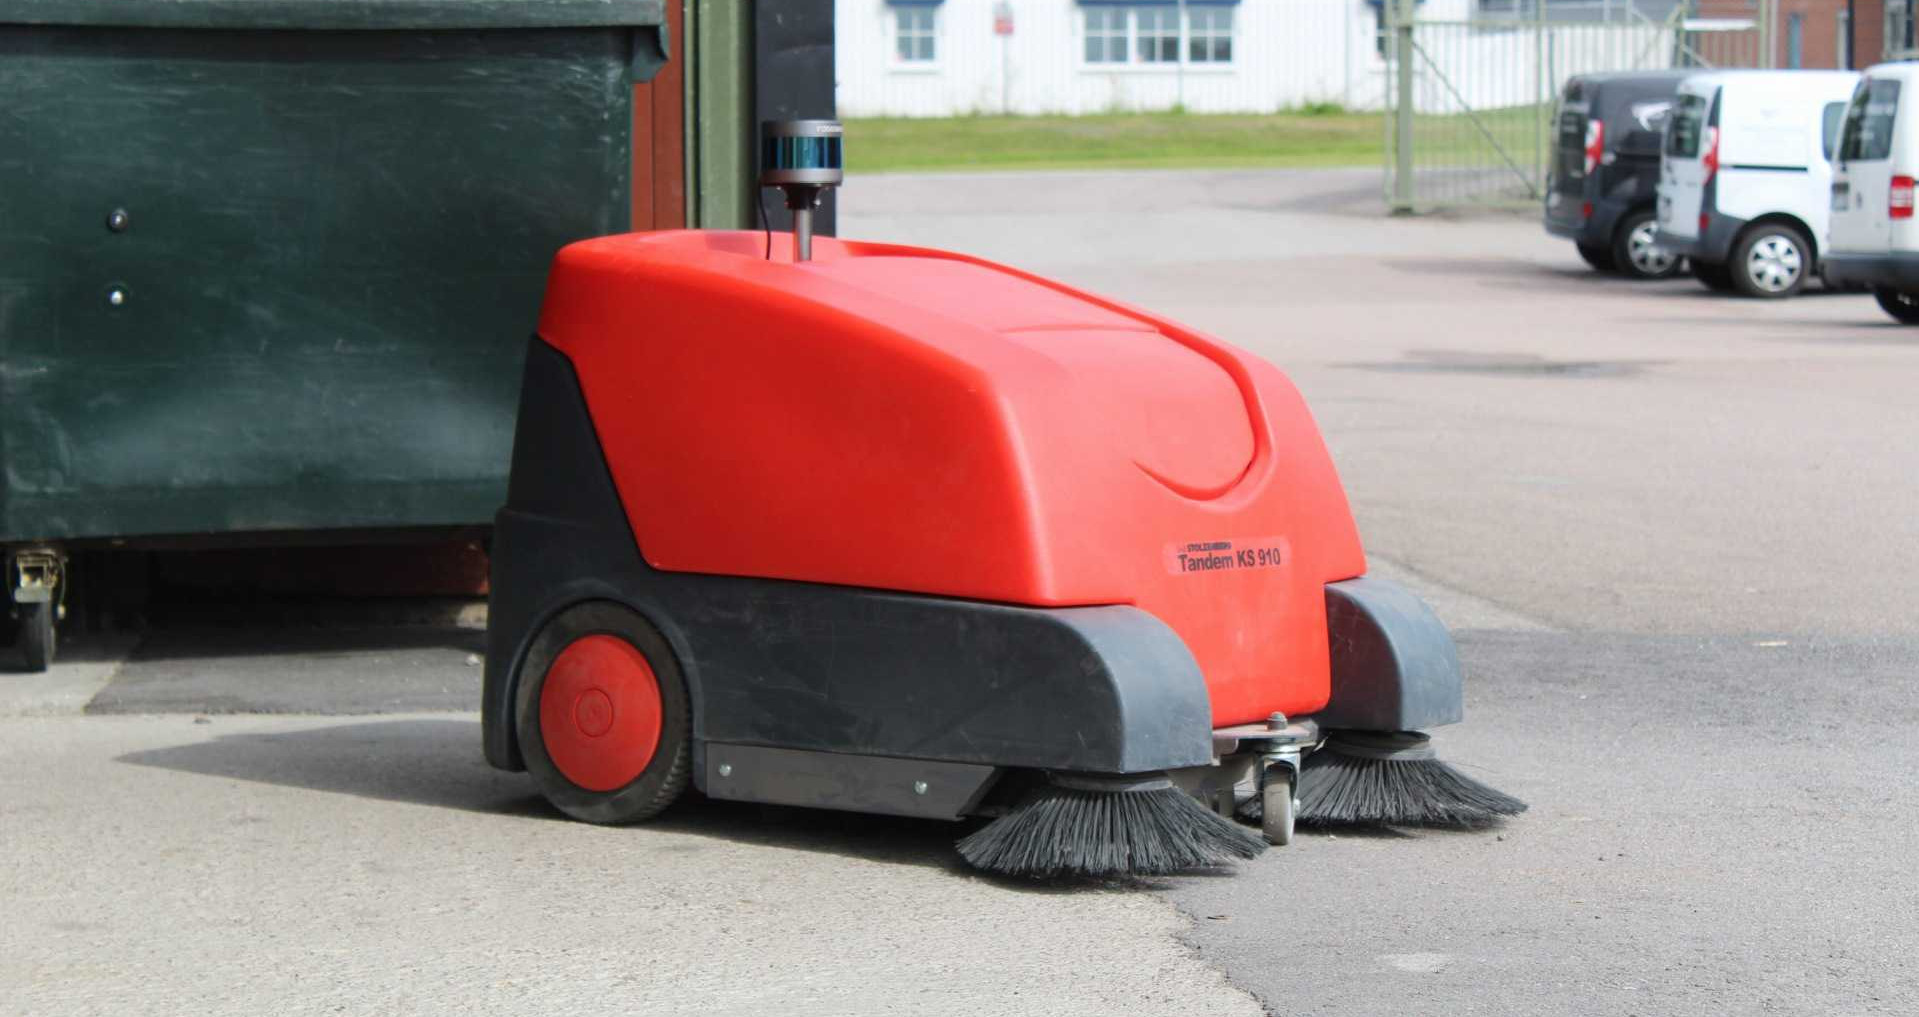
\includegraphics[width=\textwidth]{figures/sweeper_robot_cropped.jpg}
	%			%\caption{A modified Tandem KS 910 sweeping machine. }
	%			\label{fig:robot}
	%		\end{subfigure}
	%		\caption{\textbf{Top:} Garage and Highway Bridge. \textbf{Bottom:} Crossing and a robot sweeper (a modified Tandem KS 910 sweeping machine).}
	%		\label{fig:maps-and-robot}
	%	\end{figure*}
	
	\subsection{Scenario}
	\label{sec:benchmark-scenario}
	% TODO
	%	\begin{itemize}
	%		\item Description of the task.
	%		\item Robot platform with dimensions and stats (it is only a prototype and not yet operational)
	%		\item Figure of the robot
	%		\item Description of the task execution
	%		\item Description of the meta-CPP algorithm
	%	\end{itemize}
	A road sweeping robot 
	%(Figure \ref{fig:robot}) 
	of dimension
	$\text{length}~=~1m,\;\text{breadth}~=~0.75m,\;\text{height}~=~0.8m$
	%\begin{align*}
	%    \text{length} = 1m, \;\text{breadth} = 0.75m, \;\text{height} = 0.8m
	%\end{align*}
	is tasked with cleaning the ground surface in an urban environment. 
	%The robot is assumed to travel at a slow enough speed to be safely avoidable by people (beside other safety measures in place). A comfortable walking speed is between 1.2 and 1.5 m/s for adults across all ages \cite{bohannon1997comfortable}. The robot is assumed to travel at a speed of 1m/s. The robot actuators are most effective when the robot is traveling at a sufficiently slow speed, and much more effective if the robot is driven straight than if it is rotating.
	The actuators are most effective when driving straight and quickly lose effectiveness when turning wide.
	
	A 3D point cloud of the target environment is available for offline CPP. 
	%In some cases there are stationary sensors, ground or areal 3D exploration has been performed earlier by other robots or the sweeper robot itself has previously scanned the environment. Local difference between the collected point cloud and what is observed when executing the coverage path is assumed to be neglectable due to the large scales involved. Any locally-obstructive obstacle will likely have a minor effect on the overall cost of the coverage path.
	%
	Given a point cloud and a starting point, traversable and coverable points are classified and collected using terrain assessment (\ref{sec:terrain-assessment}). A maximum a posteriori (with respect to cost) path is found by optimizing a specified CPP algorithm over its parameters using Bayesian Optimization (\ref{sec:parameter-optimization}) such as HyperOpt \cite{bergstra2013making}, based on prior distributions over the parameters. The parameter optimization perform domain adaptation, and a much better path for the given domain and task is found than if an arbitrary parameter configuration is used that has not been optimized for the problem instance. This is a meta algorithm for domain adaptive offline CPP.
	The resulting path is executed by a motion planner capable of collision avoidance \cite{krusi2017driving,andersson2018receding}.%. If the environment contains dynamic obstacles then a safe motion planner which can deal with dynamic obstacles is used \cite{andersson2018receding}.
	
	%Due to the environment having complex border geometry is unreasonable to expect 100\% coverage of the actual coverable area. A planar or voxel-discretization approximation of only coverable cells would yield CPP solutions that are 100\% in the representation, but not necessarily with respect to the real coverable geometry. As long as all traversable points reach 100\% coverage then it is acceptable that the coverage for coverable points to only get close to (but not reaching) 100\%.
	
	%	\begin{figure}
	%		\centering
	%		\begin{subfigure}{\columnwidth}
	%			\centering
	%			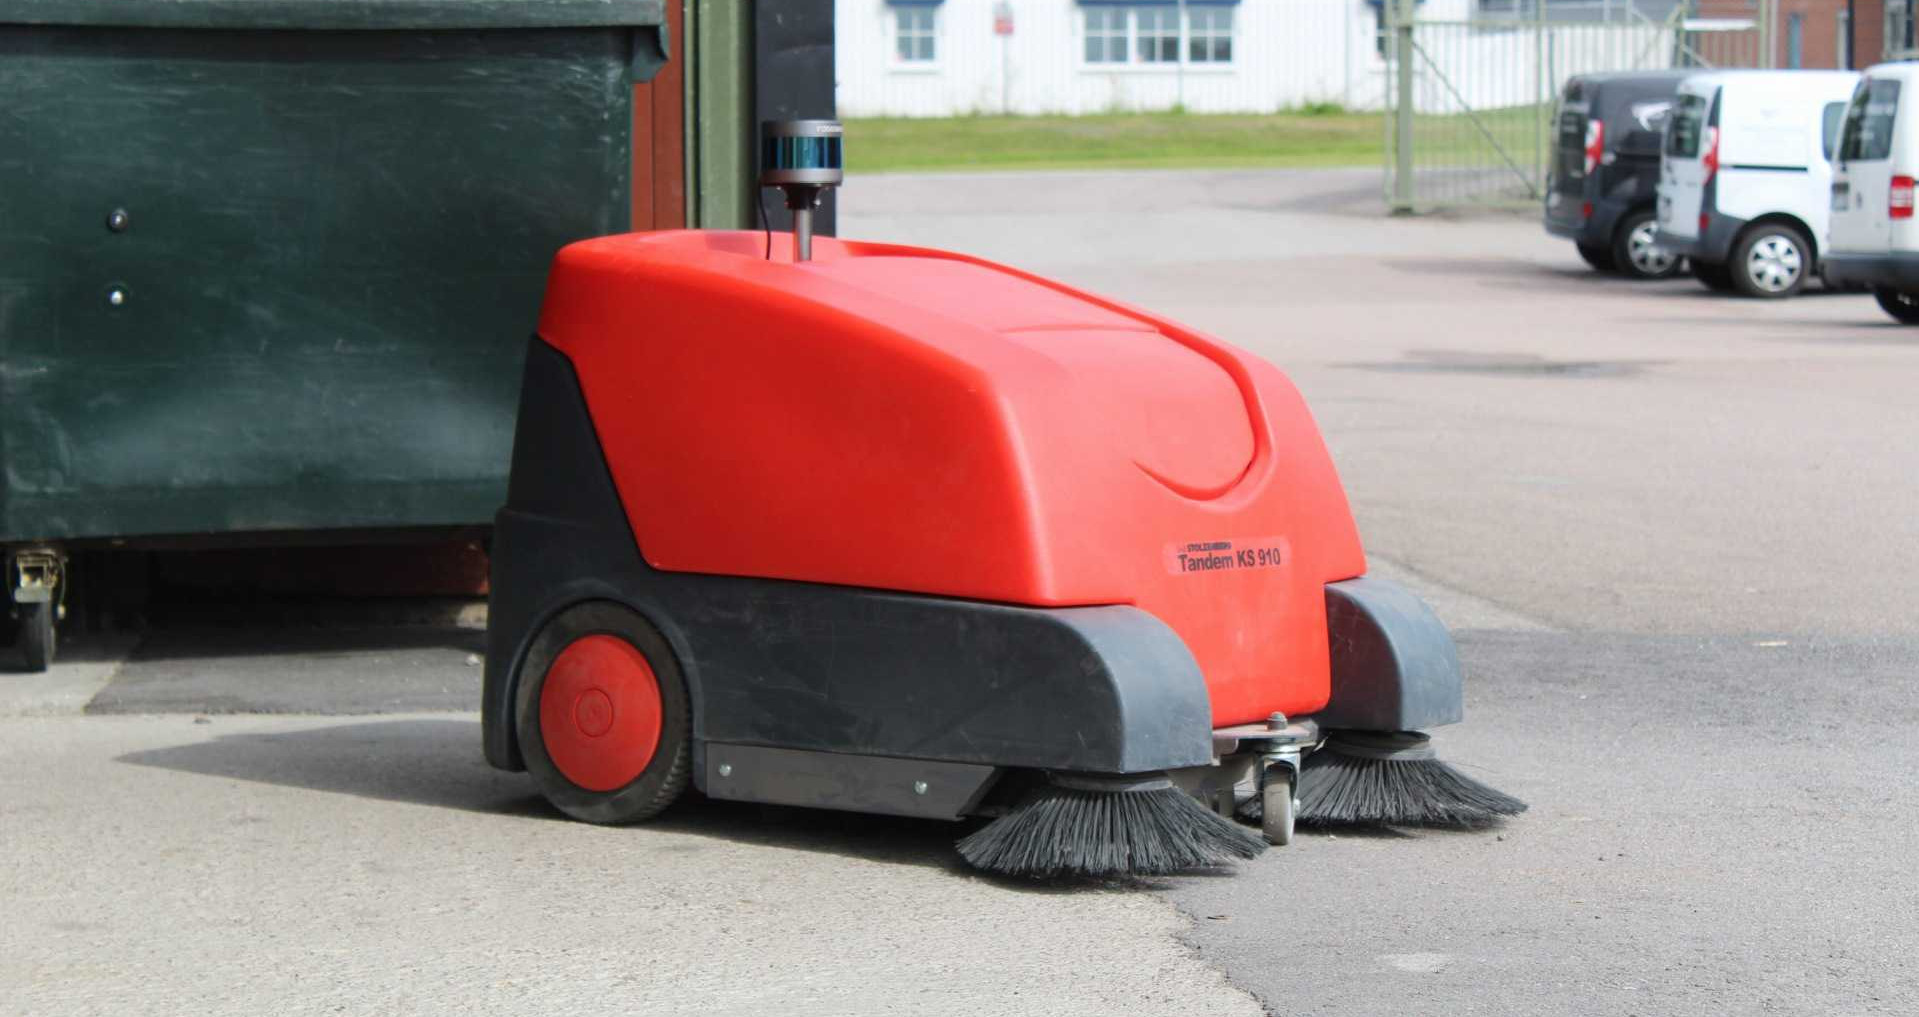
\includegraphics[width=\textwidth]{figures/sweeper_robot_cropped.jpg}
	%		\end{subfigure}
	%		\caption{Sweeper robot, a modified Tandem KS 910 sweeping machine. }
	%		\label{fig:robot}
	%	\end{figure}
	
	
	
	\section{Evaluation}
	\label{sec:evaluation}
	
	%	Parameters for the Motion Planner are presented in Table \ref{tab:mp_parameters}.
	%	\begin{table}[h!]
	%		\centering
	%		\caption{Motion Planner parameter. Values of \emph{Resolution} parameters are set to give a good resolution while keeping the computational time on a reasonable level. \emph{Hand tuned based on tests} parameters are hand tuned by making multiple tests and adjust the values to give plausible reliance, computational time and paths.}
	%		\begin{tabular}{|l|c|l|c|}
	%			\hline 
	%			\textbf{Parameter} & \textbf{Value} & \textbf{Description} & \textbf{Based on} \\
	%			\hline 
	%			$\lambda$ & 0.1 m & Step size & Resolution \\
	%			$\lambda_{A*}$ & 0.5 m & Step size used in A* & Hand tuned b.o. tests \\
	%			$\lambda_{RRT}$ & 0.3 m & Step size used in RRT & Hand tuned b.o. tests \\
	%			$r_{trav}$ & 0.2 m & Threshold for untraversability & Hand tuned b.o. tests \\
	%			$N^{RRT}_{max}$ & 10 000 & Max iterations in RRT & Resolution \\
	%			\hline 
	%		\end{tabular}
	%		
	%		\label{tab:mp_parameters}
	%	\end{table}
	
	%	\begin{figure*}[!b]
	%		\centering
	%		\begin{subfigure}{0.32\textwidth}
	%			\centering
	%			\centering
	%			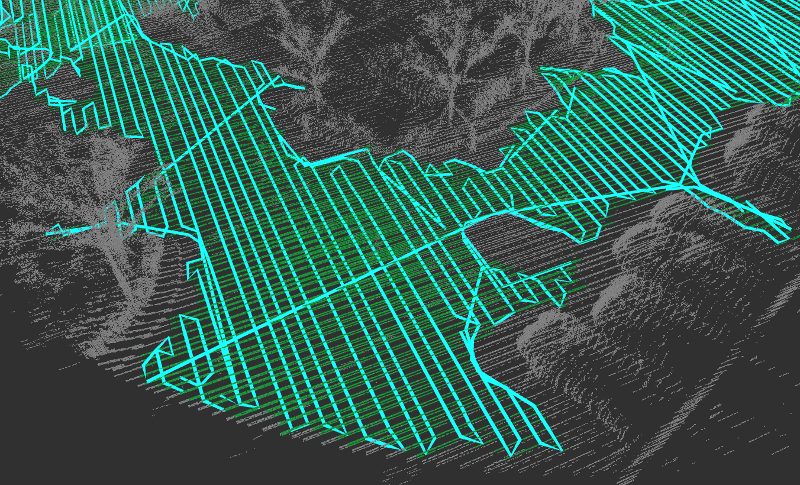
\includegraphics[width=\textwidth]{figures/example_bastar2.png}
	%			\caption{BA*}
	%			\label{fig:example_bstar}
	%		\end{subfigure}
	%		\begin{subfigure}{0.32\textwidth}
	%			\centering
	%			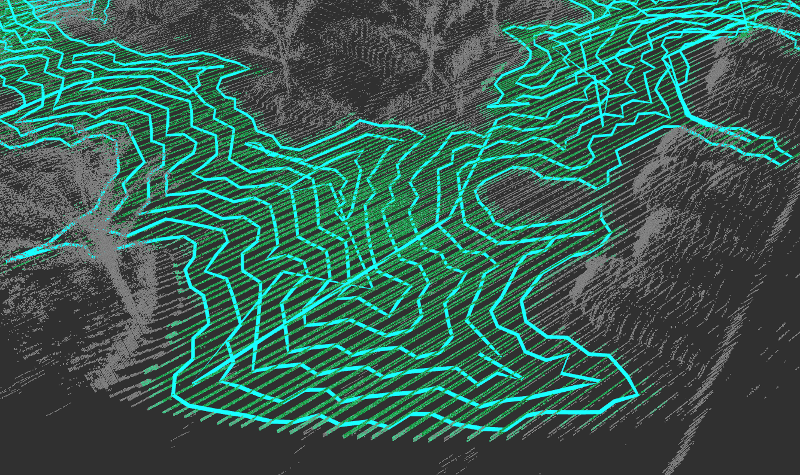
\includegraphics[width=\textwidth]{figures/example_inward_spiral.png}
	%			\caption{Inward Spiral}
	%			\label{fig:example_inward_spiral}
	%		\end{subfigure}
	%		\begin{subfigure}{0.32\textwidth}
	%			\centering
	%			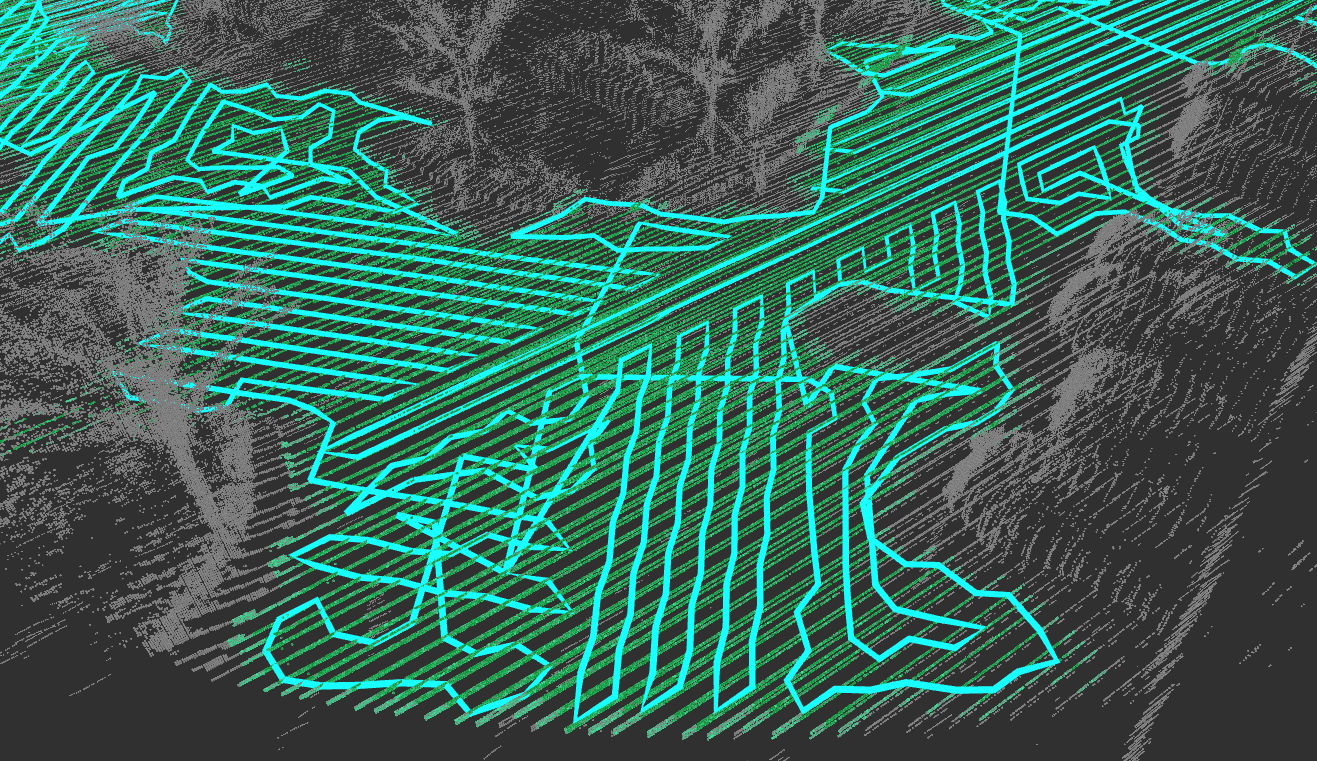
\includegraphics[width=\textwidth]{figures/example_sampled_bastar.png}
	%			\caption{Sampled BA*}
	%			\label{fig:example_sampled_bstar}
	%		\end{subfigure}
	%		\caption{Coverage paths on the Garage environment. Note XYZ special niceity of Sampled BA*.}
	%		\label{fig:algorithm_experiment_examples}
	%	\end{figure*}
	%
	%Time budget XYZ due to lower bound on area coverage by robot (traversable area divided by (robot footprint area times robot max speed)) being ABC hours.
	The CPP algorithm parameters are optimized using HyperOpt \cite{bergstra2013making} based on a single starting position per environment. Parameters are sampled from the distributions in Table \ref{tab:parameters-result}. We ran 100 evaluations of HyperOpt for each algorithm, for each environment, from the same start position. Table \ref{tab:opt-result} lists the results, where the proposed method is consistently significantly better than the other two methods in cost and rotation across all environments.  
	\begin{table}
		\centering
		\caption{CPP parameters optimized using HyperOpt on start position.}
		\begin{tabular}{|l|l|l|l|l|}
			\hline
			\multicolumn{5}{|l|}{\textbf{BA*}} \Tstrut \\
			\hline
			\textbf{Parameter} & \textbf{Garage} & \textbf{Bridge} & \textbf{Crossing} & \textbf{Prior}\Tstrut \\
			\hline
			$\lambda_{CPP}$ & 0.634m & 0.557m & 0.524m & $\mathcal{U}(0.5,1)$\Tstrut\\
			$r_{visited}$ & 0.473m & 0.453m & 0.404m & $\mathcal{U}(0.25,0.5)$\\
			$\phi$ & 4.65 rad & 5.34rad & 4.70 rad & $\mathcal{U}(0, 2\pi)$\\
			\hline
			\multicolumn{5}{|l|}{\textbf{Inwards Spiral}} \Tstrut \\
			\hline
			\textbf{Parameter} & \textbf{Garage} & \textbf{Bridge} & \textbf{Crossing} & \textbf{Prior}\Tstrut \\
			\hline
			$\lambda_{CPP}$ & 0.628m & 0.737m & 0.665 & $\mathcal{U}(0.5,1)$\Tstrut\\
			$r_{visited}$ & 0.499m & 0.483 & 0.500 & $\mathcal{U}(0.25,0.5)$\\
			\hline
			\multicolumn{5}{|l|}{\textbf{Sampled BA* \& Inwards Spiral}} \Tstrut \\
			\hline
			\textbf{Parameter} & \textbf{Garage} & \textbf{Bridge} & \textbf{Crossing} & \textbf{Prior}\Tstrut \\
			\hline
			$E^1$ & 0.865 & 0.940 & 0.863 & $\mathcal{U}(075,0.95)$\\
			$d^1_{max}$ & 4.13m & 4.49m & 1.69m & $\mathcal{U}(1,5)$\\
			$d^2_{max}$ & 6.94m & 7.06m & 4.48m & $\mathcal{U}(4,10)$\\
			$C^{1}_{min}$ & 8238 & 12773 & 6488 & *\\
			$C^{2}_{min}$ & 13645 & 25989 & 8141 & **\\
			$\lambda_{CPP}$ & 0.548m & 0.619m & 0.554 & $\mathcal{U}(0.5,1)$\Tstrut\\
			$r_{visited}$ & 0.373 & 0.389m & 0.258 & $\mathcal{U}(0.25,0.5)$\\
			\hline 
			\multicolumn{5}{l}{* Based on coverable area $A$: $\mathcal{U}(0.165A,0.33A)$} \\
			\multicolumn{5}{l}{** Based on coverable area $A$: $\mathcal{U}(0.33A,0.66A)$}
		\end{tabular}
		\label{tab:parameters-result}
	\end{table}
	\begin{table}
		\centering
		\caption{Result of meta-CPP domain adapted solution.}
		\begin{tabular}{|l|l|l|l|l|}
			\hline
			\textbf{Environment} &\textbf{Algorithm} & \textbf{Cost} & \textbf{Length} & \textbf{Rotation}\Tstrut\\
			\hline
			Garage & Sampled BA*\dots& \textbf{4077} &	2999&	\textbf{1078}\Tstrut\\
			& BA* & 4238&	\textbf{2896}&	1342\\
			& Inwards Spiral & 5787&	3101&	2686\\
			\hline
			Bridge & Sampled BA*\dots & \textbf{5797}&	4643&	\textbf{1154}\Tstrut\\
			& BA* & 6385&	4562&	1823\\
			& Inwards Spiral & 7213&	\textbf{4440}&	2773\\
			\hline
			Crossing & Sampled BA*\dots & \textbf{3001}&	\textbf{2186}&	\textbf{815}\Tstrut\\
			& BA* & 3262&	2249&	1013\\
			& Inwards Spiral & 4054&	2239&	1815\\
			\hline 
		\end{tabular}
		\label{tab:opt-result}
	\end{table}
	%
	To evaluate the robustness of the domain adaptation to other starting positions, i.e. measure the generalization of the MAP parameters, another 10 start points are randomized for respective environment and solved using all three algorithms. The results are presented in Figure \ref{fig:result-cost-coverage}, where the proposed algorithm still outperforms BA* and Inward Spiral, apart from for the highest degree of coverage on Two-storey Garage. Examples are shown in Figure \ref{fig:algorithm_experiment_examples}.
	
	%$C^{1}_{min}$ & 8238 & 12773 & 6488 & $\mathcal{U}(5\text{E}3,1\text{E}4)$\\
	%$C^{2}_{min}$ & 13645 & 25989 & 8141 & $\mathcal{U}(1\text{E}4,2\text{E}4)$\\
	
	
	
	
	\section{Conclusions}
	\label{sec:conclusions}
	A realistic benchmark suite for advancing the CPP capabilities of service robot tasks in urban environtnments is presented, together with a novel state-of-the-art algorithm which combine the strengths of three other prominent CPP algorithms. A rigid domain adaptation methodology for CPP is proposed, and the generalization of the domain adaptation is demonstrated in the evaluation. Using Bayesian optimization we optimize the non-exact CPP algorithms for the best possible path they can generate.
	%
	The next step towards field robotics is to evaluating the proposed algorithm and domain adaptation approach in practice onboard a real robot sweeper.
	%\begin{itemize}
	%		\item Compare with learning-based methods: A* search and learned heuristic.
	%		\item Future work: Real experiments in varied garage maps when sweeper robot prototype is operational.
	%	\end{itemize}
	
	%%%%%%%%%%%%%%%%%%%%%%%%%%%%%%%%%%%%%%%%%%%%%%%%%%%%%%%%%%%%%%%%%%%%%%%%%%%%%%%%
	%\section*{APPENDIX}
	
	
	%\section*{ACKNOWLEDGMENT}
	%
	%The preferred spelling of the word �acknowledgment� in America is without an �e� after the �g�. Avoid the stilted expression, �One of us (R. B. G.) thanks . . .�  Instead, try �R. B. G. thanks�. Put sponsor acknowledgments in the unnumbered footnote on the first page.
	
	
	\clearpage
	%%%%%%%%%%%%%%%%%%%%%%%%%%%%%%%%%%%%%%%%%%%%%%%%%%%%%%%%%%%%%%%%%%%%%%%%%%%%%%%%
	\bibliographystyle{IEEEtran}
	\bibliography{bibliography}
	
	
	
\end{document}
